
\chapter{供给与需求的市场力量}

\keyword{供给}与\keyword{需求}是经济学家最经常使用的两个词。
供给与需求是使市场经济运行的力量。
它们决定了每种物品的产量及其出售的价格。
如果你想知道一件事件或政策如何影响经济,
你就应该先考虑它将如何影响供给和需求。


\section{市场与竞争}

供给与需求是指人们在竞争市场上互相交易时的行为。

\subsection{什么是市场}

市场是由某种物品或服务的买者与卖者组成的一个群体。
买者作为一个群体决定了一种产品的需求,
而卖者作为一个群体决定了一种产品的供给。


\subsection{什么是竞争}

经济学家用\keyword{竞争市场}来描述有许多买者与卖者并且每一个人对市场价格的影响都微乎其微的市场。


\keyword{完全竞争}的市场必须具备两个特征:
\begin{itemize}
\item 可供销售的物品是完全相同的。
\item 买者和卖者人数众多,以至于没有任何一个买者或卖者可以影响市场价格。
\end{itemize}
由于完全竞争市场上的买者与卖者都必须接受市场决定的价格,
所以他们被成为\keyword{价格接受者}。


并不是所有物品与服务都在完全竞争市场上出售。
一些市场只有一个卖者,
而且这个卖者决定价格,
这样的卖者被称为\keyword{垄断者}。


\section{需求}

\subsection{需求曲线:价格和需求量之间的关系}

一种物品的\keyword{需求量}是买者愿意并且能够购买的该种物品的数量。

需求定理:在其他条件不变时,一种物品的价格上升,对该物品的需求量减少;
一种物品的价格下降,对该物品的需求量增加。

\begin{figure}[!ht]
  \centering
  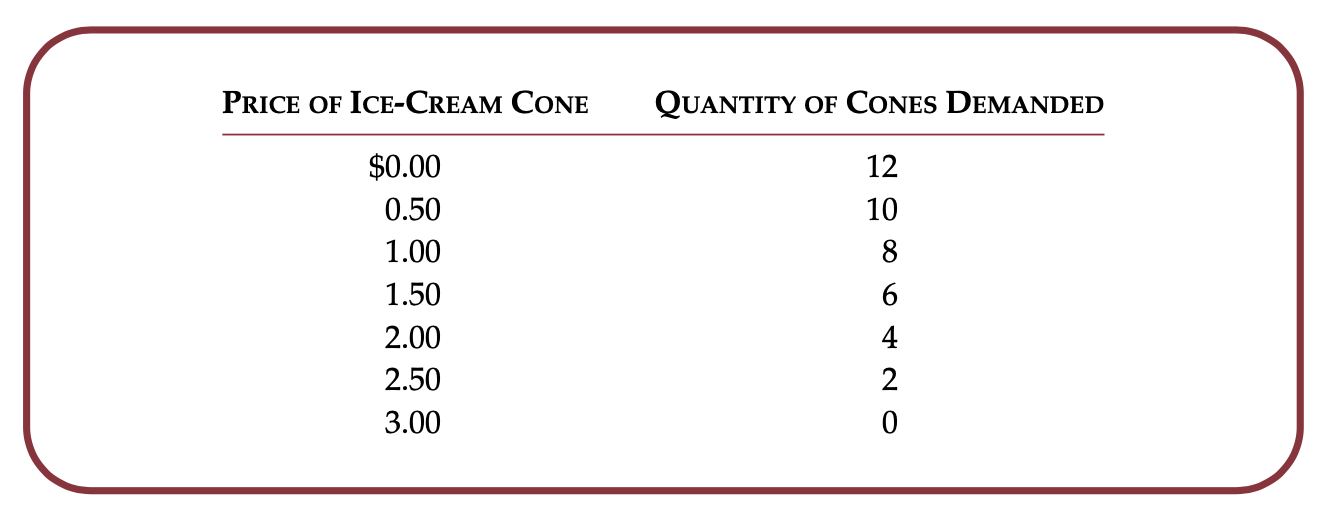
\includegraphics[width=\textwidth]{pics/demand-schedule}
  \caption{需求表}
  \label{fig:demand-schedule}
\end{figure}

表\ref{fig:demand-schedule}是一个需求表,
它表明在影响消费者想购买的数量的其他因素都保持不变的情况下,
一种物品的价格与其需求量之间的关系。

\begin{figure}[!ht]
  \centering
  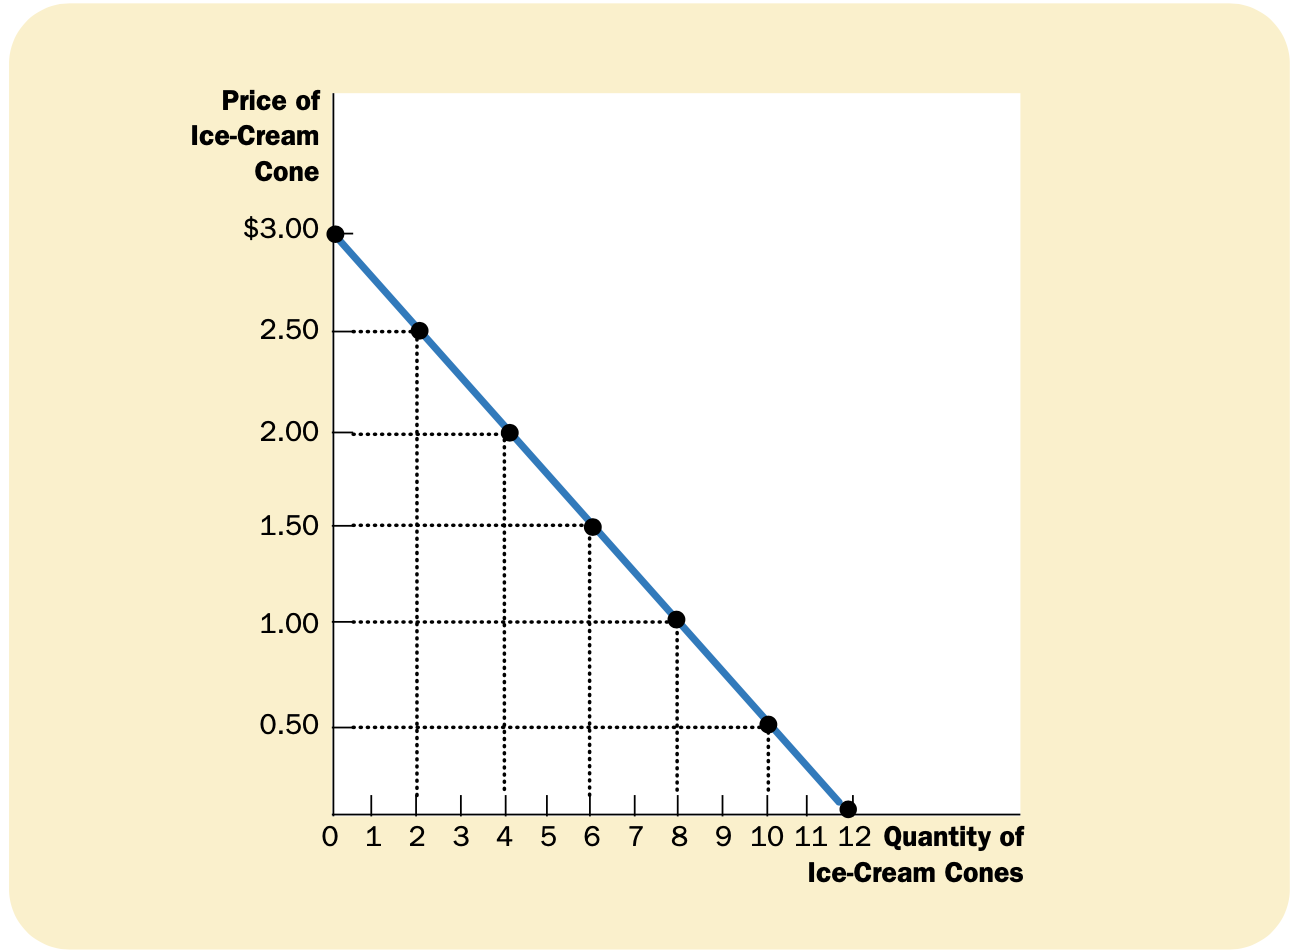
\includegraphics[width=\textwidth]{pics/demand-curve}
  \caption{需求曲线}
  \label{fig:demand-curve}
\end{figure}

图\ref{fig:demand-curve}表示需求曲线,
它把价格和需求量联系在一起。


\subsection{市场需求与个人需求}

市场需求是所有个人对某种特定物品或服务的需求的总和。


\subsection{需求曲线的移动}

由于市场需求曲线假设其他条件不变,
但随着时间的推移,
该曲线不一定是稳定的,
如果某个因素改变了任何一种既定价格水平的需求量,
需求曲线就会移动。


有许多变量会是需求曲线移动。
以下是一些最重要的变量:
\begin{itemize}
\item 收入
\item 相关物品的价格
\item 爱好
\item 预期
\item 买者的数量
\end{itemize}

当收入减少时,如果一种物品的需求量减少,这种物品就被称为\keyword{正常物品}。
当收入减少时,如果一种物品的需求量增加,这种物品就被称为\keyword{低档物品}。
当一种物品价格下降一起对另一种物品的需求量减少时,这种物品就被称为\keyword{替代品}。
当一种物品价格下降一起对另一种物品的需求量增加时,这种物品就被称为\keyword{互补品}。


\section{供给}

\subsection{供给曲线:价格与供给量之间的关系}

一种物品或者服务的\keyword{供给量}是卖者愿意并且能够出售的该种物品的数量。

供给定理:在其他条件不变时,一种物品价格上升,该物品供给增加;
一种物品价格下降,该物品供给减少。

供给表:在影响某种物品的生产者想出售数量的其他因素都保持不变的情况下,
该物品的价格和供给量之间的关系。

供给曲线:把价格和供给量联系在一起的曲线。



\subsection{市场供给与个人供给}

市场供给是所有卖者供给的总和。


\subsection{供给曲线的移动}


由于市场供给曲线假设其他条件不变,
当这些因素中的一个因素变动时,
该曲线将会发生移动。



有许多变量会使供给曲线移动,
以下是一些最重要的变量:
\begin{itemize}
\item 投入品价格
\item 技术
\item 预期
\item 卖者的数量
\end{itemize}


\section{供给与需求的结合}

\subsection{均衡}

\begin{figure}[!ht]
  \centering
  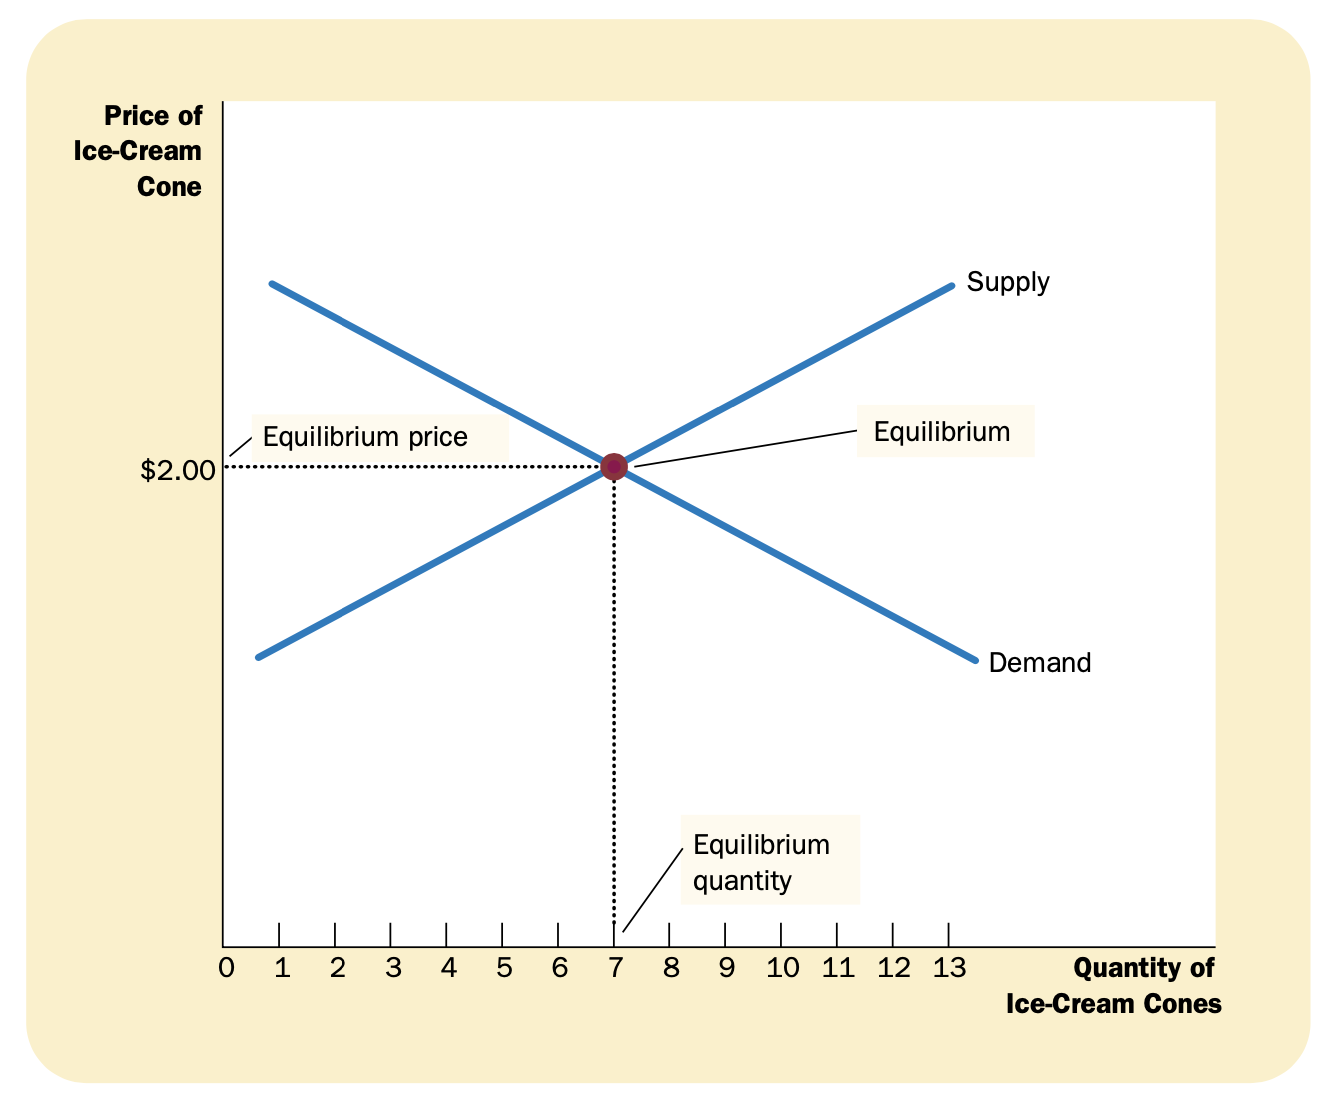
\includegraphics[width=\textwidth]{pics/equilibrium-of-supply-and-demand}
  \caption{供给与需求的均衡}
  \label{fig:equilibrium-of-supply-and-demand}
\end{figure}

图\ref{fig:equilibrium-of-supply-and-demand}同时给出了市场供给曲线和市场需求曲线。
供给曲线和需求曲线相较于一点,这一点被称为市场的\keyword{均衡}。
这两条曲线相交时的价格被称为\keyword{均衡价格},
而相交时的数量被称为\keyword{均衡数量}。


供求定理:任何一种物品的价格都会自发调整,使该物品的供给与需求达到平衡。


\subsection{分析均衡变动的三个步骤}

供给和需求共同决定了市场均衡,
市场均衡又决定了物品价格,
以及买者所购买和卖者所生产的该物品数量。
均衡价格和均衡数量取决于供给曲线和需求曲线的位置。
当某些事件使一种一条曲线移动时,
市场上的均衡就改变了,
从而将在买者和卖者之间产生新的均衡价格和均衡数量。



当分析某个事件如何影响一个市场上的均衡的时候,
我们按三个步骤进行:
\begin{enumerate}
\item 确定该事件是使供给曲线还是需求曲线移动,还是使两条曲线都移动。
\item 确定曲线是向右移动,还是向左移动。
\item 用供求图来比较原来的均衡和新均衡,以说明这种移动如何影响均衡价格和均衡数量。
\end{enumerate}


供给曲线的移动被称为“供给变动”,
而需求曲线的移动被称为“需求变动”。
沿着一条固定供给曲线的变动称为“供给量的变动”,
而沿着一条固定需求曲线的变动称为“需求量的变动”。


\begin{tcolorbox}
  哄抬物价是变相抢劫吗?

  道德掺合进经济学里对法律肯定是有害的。
  只有在需求的物品出现短缺的情况下,哄抬物价才会出现。
  如果没有短缺,正常的市场过程会阻止物价突然上升。

  在极端需求情况下允许价格上涨限制了过度消费。
  人们会更仔细地考虑他们的购买。
  结果在极端的情况下会又更多的顾客买得到物品。
  市场过程的结果实际上比反哄抬物价更能实现较为平等的分配。

  商人实际上并没有从灾难中获利,
  商人是通过对物价的管理来获利的,
  这种对自己物价的管理实际上扩大了商品的分配范围,
  并限制了囤积居奇,
  从而产生了有益的社会效应。
  简言之,他们是由于提供了重要的公共服务而正当地获得了回报。
\end{tcolorbox}


\section{价格如何配置资源}

供给和需求共同决定了经济中许多不同物品与服务的价格,
而价格又是引导资源配置的信号。
在市场经济中,价格是配置稀缺资源的机制。






